\begin{filecontents*}{references.bib}
@misc{kaggle_tribunal,
  author = {Shengxue, S.},
  title = {League of Legends Tribunal Chatlogs},
  year = {2020},
  howpublished = {\url{https://www.kaggle.com/datasets/simshengxue/league-of-legends-tribunal-chatlogs}},
  note = {Kaggle}
}

@inproceedings{toxic_chat_rg,
  author = {Lee, Jaehong and Rerkjirattikal, Pavinee and Nam, Sanggyu},
  title = {Toxic Chat Detection in Online Games Using Hybrid {BERT} and Character-level {CNN}},
  booktitle = {Proceedings of the MakeLearn, TIIM \& PIConf International Conference},
  year = {2025},
  address = {Bangkok, Thailand},
  note = {Available: \url{https://www.researchgate.net/publication/393480032_Toxic_Chat_Detection_in_Online_Games_Using_Hybrid_BERT_and_Character-level_CNN}}
}

@misc{jigsaw,
  author = {Jigsaw and Google},
  title = {Toxic Comment Classification Challenge},
  year = {2018},
  howpublished = {\url{https://www.kaggle.com/competitions/jigsaw-toxic-comment-classification-challenge}},
  note = {Kaggle}
}

@inproceedings{davidson2017,
  author = {Davidson, Thomas and Warmsley, Dana and Macy, Michael and Weber, Ingmar},
  title = {Automated Hate Speech Detection and the Problem of Offensive Language},
  booktitle = {Proceedings of the 11th International AAAI Conference on Web and Social Media (ICWSM)},
  year = {2017}
}

@inproceedings{kwak2015,
  author = {Kwak, Haewoon and Blackburn, Jeremy and Han, Seungyeop},
  title = {Exploring Cyberbullying and Other Toxic Behavior in Team Competition Online Games},
  booktitle = {Proceedings of the 33rd Annual ACM Conference on Human Factors in Computing Systems (CHI)},
  year = {2015}
}

@article{hochreiter1997,
  author = {Hochreiter, Sepp and Schmidhuber, J\"{u}rgen},
  title = {Long Short-Term Memory},
  journal = {Neural Computation},
  volume = {9},
  number = {8},
  pages = {1735--1780},
  year = {1997}
}
\end{filecontents*}

\documentclass[final]{article}

\usepackage{APS360}
\usepackage[utf8]{inputenc}    % allow utf-8 input
\usepackage[T1]{fontenc}       % use 8-bit T1 fonts
\usepackage{hyperref}          % hyperlinks
\usepackage{url}               % simple URL typesetting
\usepackage{booktabs}          % professional-quality tables
\usepackage{amsfonts}          % blackboard math symbols
\usepackage{nicefrac}          % compact symbols for 1/2, etc.
\usepackage{microtype}         % microtypography
\usepackage{xcolor}            % colors
\usepackage{graphicx}          % required for inserting actual images later
 
\title{LoL Toxic Gaming Chat Classifier}

\author{%
  Alex You \\
  1011175185, alex.you@mail.utoronto.ca\\
   \href{https://colab.research.google.com/drive/118GzPaV2duFgdaWv7MNPaimFRUn4lxQw?usp=sharing}{Link to Google Colab}\\
}

\begin{document}

\maketitle

\vspace{-0.5in}

\section*{Introduction}

Online gaming communities, particularly in the largest competitive multiplayer video game League of Legends (LoL), are notorious for toxic chat. While toxicity is heavily penalized with account restrictions, automated moderation tools frequently fail because they are trained on general internet text, lacking an understanding of highly contextual gaming lingo (ex. "inting" or "jg diff"). This project aims to develop a domain-specific deep learning model to accurately classify toxic and non-toxic in-game LoL chat. Sequential modeling is optimal for this task, as identifying toxicity requires understanding the contextual arrangement and emotional flow of sentences, which traditional models struggle to capture.

\section*{Illustration}
Figure \ref{fig:architecture} illustrates the high-level architecture of the proposed text classification pipeline, from raw chat input to the final toxicity classification.

\begin{figure}[!h]
  \centering
  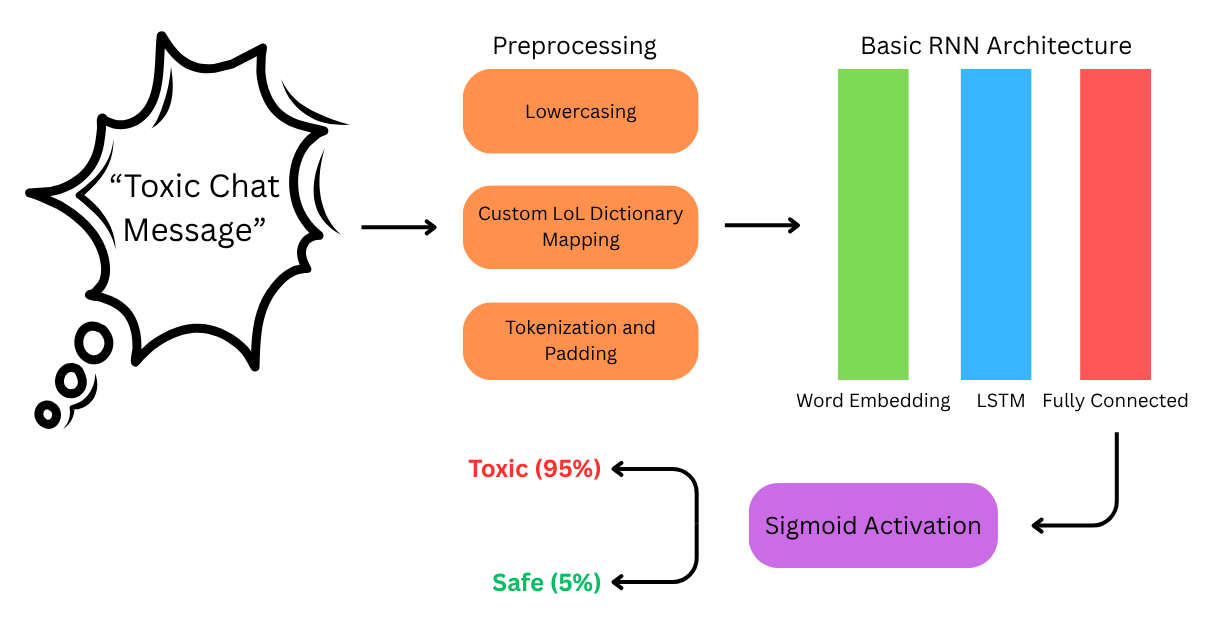
\includegraphics[width=0.8\textwidth]{APS360 Project Figure.png}
  \caption{Proposed model architecture mapping raw chat logs to a binary toxicity classification.}
  \label{fig:architecture}
\end{figure}

\section*{Background \& Related Work}

I will draw on several works to conceptualize this project. The Jigsaw Toxic Comment Challenge \cite{jigsaw} provides a standard for general toxicity detection, highlighting the need for domain-specific fine-tuning. Davidson et al. \cite{davidson2017} differentiate general offensive language from targeted hate speech, which is vital for defining "toxic" thresholds. Kwak et al. \cite{kwak2015} analyze cyberbullying specifically in LoL, offering sociological context. For architecture, Hochreiter and Schmidhuber's foundational paper on LSTMs \cite{hochreiter1997} demonstrates their effectiveness for sequential text classification. Finally, recent work using hybrid models for toxic game chat \cite{toxic_chat_rg} validates the need for context-aware neural architectures over standard baselines.

\section*{Data Processing}

This project's primary dataset is the Kaggle "LoL Tribunal Chatlogs" \cite{kaggle_tribunal}, containing thousands of reported messages. Extensive preprocessing is required for this user-generated text, such as extracting chat lines and repurposing their associated verdicts (punished vs. pardoned) as binary "toxic" or "safe" labels. Text will be lowercased, stripped of non-ASCII and spam characters, and passed through a custom dictionary to standardize LoL abbreviations (ex. "jg" to "jungle"). Finally, the text will be tokenized and padded to a fixed sequence length for efficient batching into PyTorch tensors.

\section*{Architecture}

The model will implement a Recurrent Neural Network (RNN) using Long Short-Term Memory (LSTM) cells. An Embedding layer will convert tokenized words into dense vectors, feeding into 1-2 LSTM layers designed to capture sequential context. The final hidden state will pass through a Fully Connected (Linear) layer and a Sigmoid activation to output a final toxicity probability between 0 and 1.

\section*{Baseline Model}

To evaluate this approach, I will compare the LSTM against a Support Vector Machine (SVM) trained on Term Frequency-Inverse Document Frequency (TF-IDF) features from the cleaned dataset. This standard baseline ignores word order, allowing us to measure the exact value of the LSTM's sequential awareness.  

\section*{Ethical Considerations}

Deploying automated moderation raises some ethical concerns. The Tribunal dataset is inherently biased, containing only peer-reported games, risking the amplification of the player base's historical biases. Rapidly evolving gaming lingo means that models trained on historical data might falsely flag benign new phrases. Finally, the training labels rely on the subjective, potentially flawed judgment of historical reviewers lacking full game context, rather than an objective truth.


In the preparation of this proposal, the large language model Google Gemini was utilized as an assistive tool to format and generate the BibTeX citations for the bibliography.

\bibliographystyle{IEEEtran}
\bibliography{references}

\end{document}